\documentclass[11pt]{article}

\title{ExploitFarm}
\usepackage{graphicx}
\usepackage[utf8]{inputenc}
\usepackage{hyperref}
\usepackage{float}
\usepackage[left=2.5cm, right=2.5cm, top=2.5cm, bottom=2.5cm]{geometry}
\usepackage{titlesec}
\usepackage{tocloft} % Optional: to customize TOC appearance

% Redefine paragraph to behave like a subsection for TOC purposes
\titleformat{\paragraph}
  [runin] % Keep the paragraph style without line break
  {\normalfont\normalsize\bfseries} % Style
  {\theparagraph} % Numbering style
  {1em}
  {}

\titlespacing*{\paragraph}{0pt}{3.25ex plus 1ex minus .2ex}{1em}

\setcounter{secnumdepth}{4}
\setcounter{tocdepth}{4}
\author{Domingo Dirutigliano}


\begin{document}

\begin{titlepage}
   \begin{center}
       \vspace*{1cm}

       \LARGE{\textbf{ExploitFarm Project}}

       \vspace{0.5cm}
        Analisi di progetto e documentazione
       
       \vspace{0.5cm}
       
       \begin{figure}[H]
    		\centering
    		
\includegraphics[width=0.2\textwidth]{logo.png}
		\end{figure}
       
       \vspace{0.5cm}

       \textbf{Domingo Dirutigliano}

       \vfill
            
       Politecnico di Bari\\
       Software Engineering
            
       \vspace{0.1cm}
   \end{center}
\end{titlepage}

\tableofcontents
\newpage

\section{Introduzione}
\subsection{Descrizione generale}
	"Exploitfarm" è un software completamente dedicato alle competizioni CTF Attack/Defence, che si occupa principalmente di gestire la fase di attacco e ti tutto quello che conseguentemente questa fase richiede per essere eseguita correttamente, al fine di semplificare e velocizzare gli attacchi.\\
	In generale Exploitfarm si occupa di attaccare in parallelo una serie di team (attacker) e di raccogliere ed inviare seguendo i criteri e limitazioni indicate per la competizione che si sta svolgendo le flag al gameserver (submitter).
\subsection{Obiettivi}
\begin{itemize}
    \item Setup e installazione facile, veloce, personalizzabile e facilmente automizzabile
    \item Gestione delle risorse per gli attacchi dinamica e reattiva
    \item Scrittura degli exploit e dei test su questi semplificata
    \item Interfaccia intuitiva con avvio e configurazione intuitiva e rapida
    \item Keep track of anything: accumula dati sugli attacchi e ne permette un'analisi veloce ed intuitiva
    \item Rende semplice la condivisione/collaborazione sugli attacchi e la loro esecuzione
    \item Leggero da eseguire su qualsiasi piattaforma
    \item Gestione distribuita degli attacchi
    \item Configurazione e modifiche dinamiche
\end{itemize}
\subsection{Perchè lo sviluppo di un nuovo attacker/submitter?}
Gli attacker attualmente esistenti sono spesso incompleti, difficili da configurare e da completarne il setup, facilmente inclini ad errori che spesso comportano una perdita di tempo aggiuntiva, non hanno alcun tipo di gestione del carico supportato dalla macchina che esegue gli attacchi, non memorizza o espone alcun dato statistico sull'andamento degli attacchi ed infine non gestisce la condivisione degli exploit stessi.\\
Date le forti lacune presenti in software simili già esistenti, ho ritenuto opportuno la creazione di un'alternativa agli attacker attualmente esistenti.\\
\textbf{NOTA}: "ExploitFarm" è liberamente ispirato ad un altro attacker molto famoso chiamato \href{https://github.com/DestructiveVoice/DestructiveFarm}{DestructiveFarm}, ma ne condivide a livello di codice unicamente delle piccole porzioni del suo client "start\_xploit.py" a loro volta modificate ed adattate, in alcune parti riscritte e riprogettate completamente date le netti differenze di requisiti dei progetti.
\section{Specifiche}
\subsection{Composizione del progetto}
Il progetto è composto principalmente da un server centrale (nello specifico un web server) che coordinerà una serie di client sia frontend (web) che tramite una CLI. La parte di coordinamento, di submitting e gestione dei dati è affidata al server.
    \begin{figure}[H]
    	\centering
    	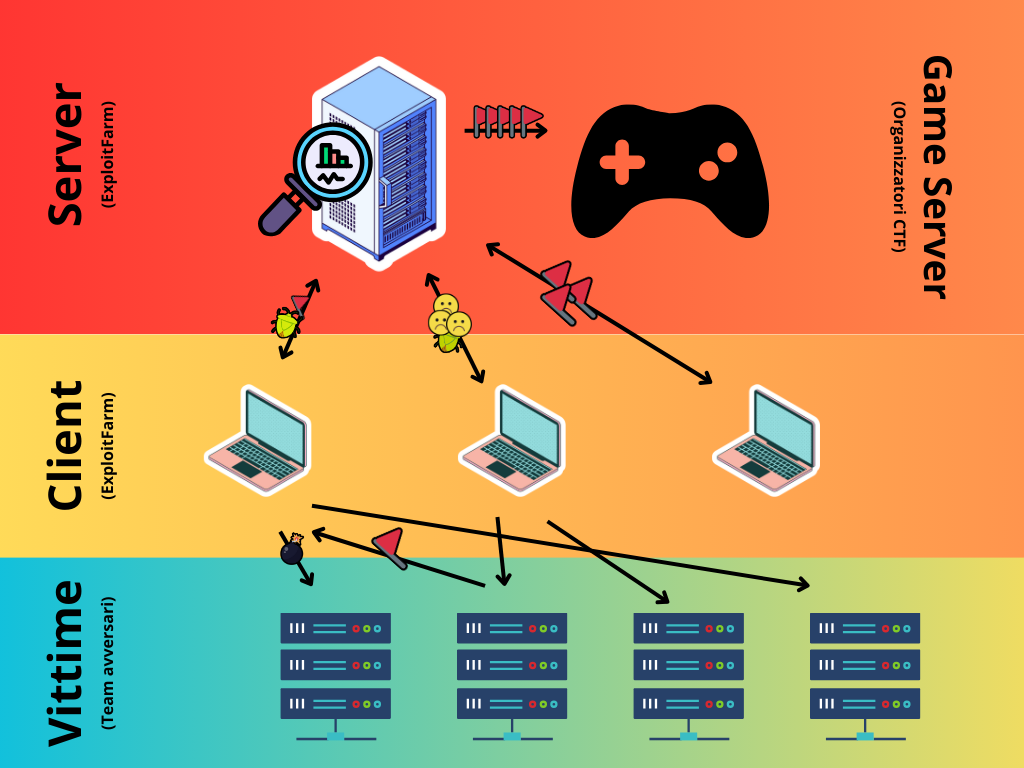
\includegraphics[width=0.8\textwidth]{general_layout.png}
	\end{figure}
\subsubsection{Backend}
Il backend sarà il core del progetto poiché conterrà tutta la logica per il coordinamento dei vari client che invieranno il risultato degli attacchi, dovrà gestire i dati ed elaborarli al fine di renderli facilmente fruibili dai client, inoltre conterrà la logica e si occuperà della gestione del submitting delle flag al gameserver seguendo i requisiti indicati in fase di setup.
\subsubsection{Frontend}
La visualizzazione avanzata dello stato di ExploitFarm è invece affidata alla parte frontend del webserver che dovrà permettere un facile accesso ai dati presenti sul server, offrendoli tramite strumenti di analisi come grafici che devono essere mirati sulle esigenze decisionali che possono emergere durante una competizione Attack Defence. Inoltre dovrà segnalare e rendere facilmente e tempestivamente nota la presenza di eventuali errori di qualsiasi tipo sull'intera infrastruttura permettendone un'intervento quanto più immediato da parte del team.
    \begin{figure}[H]
    	\centering
    	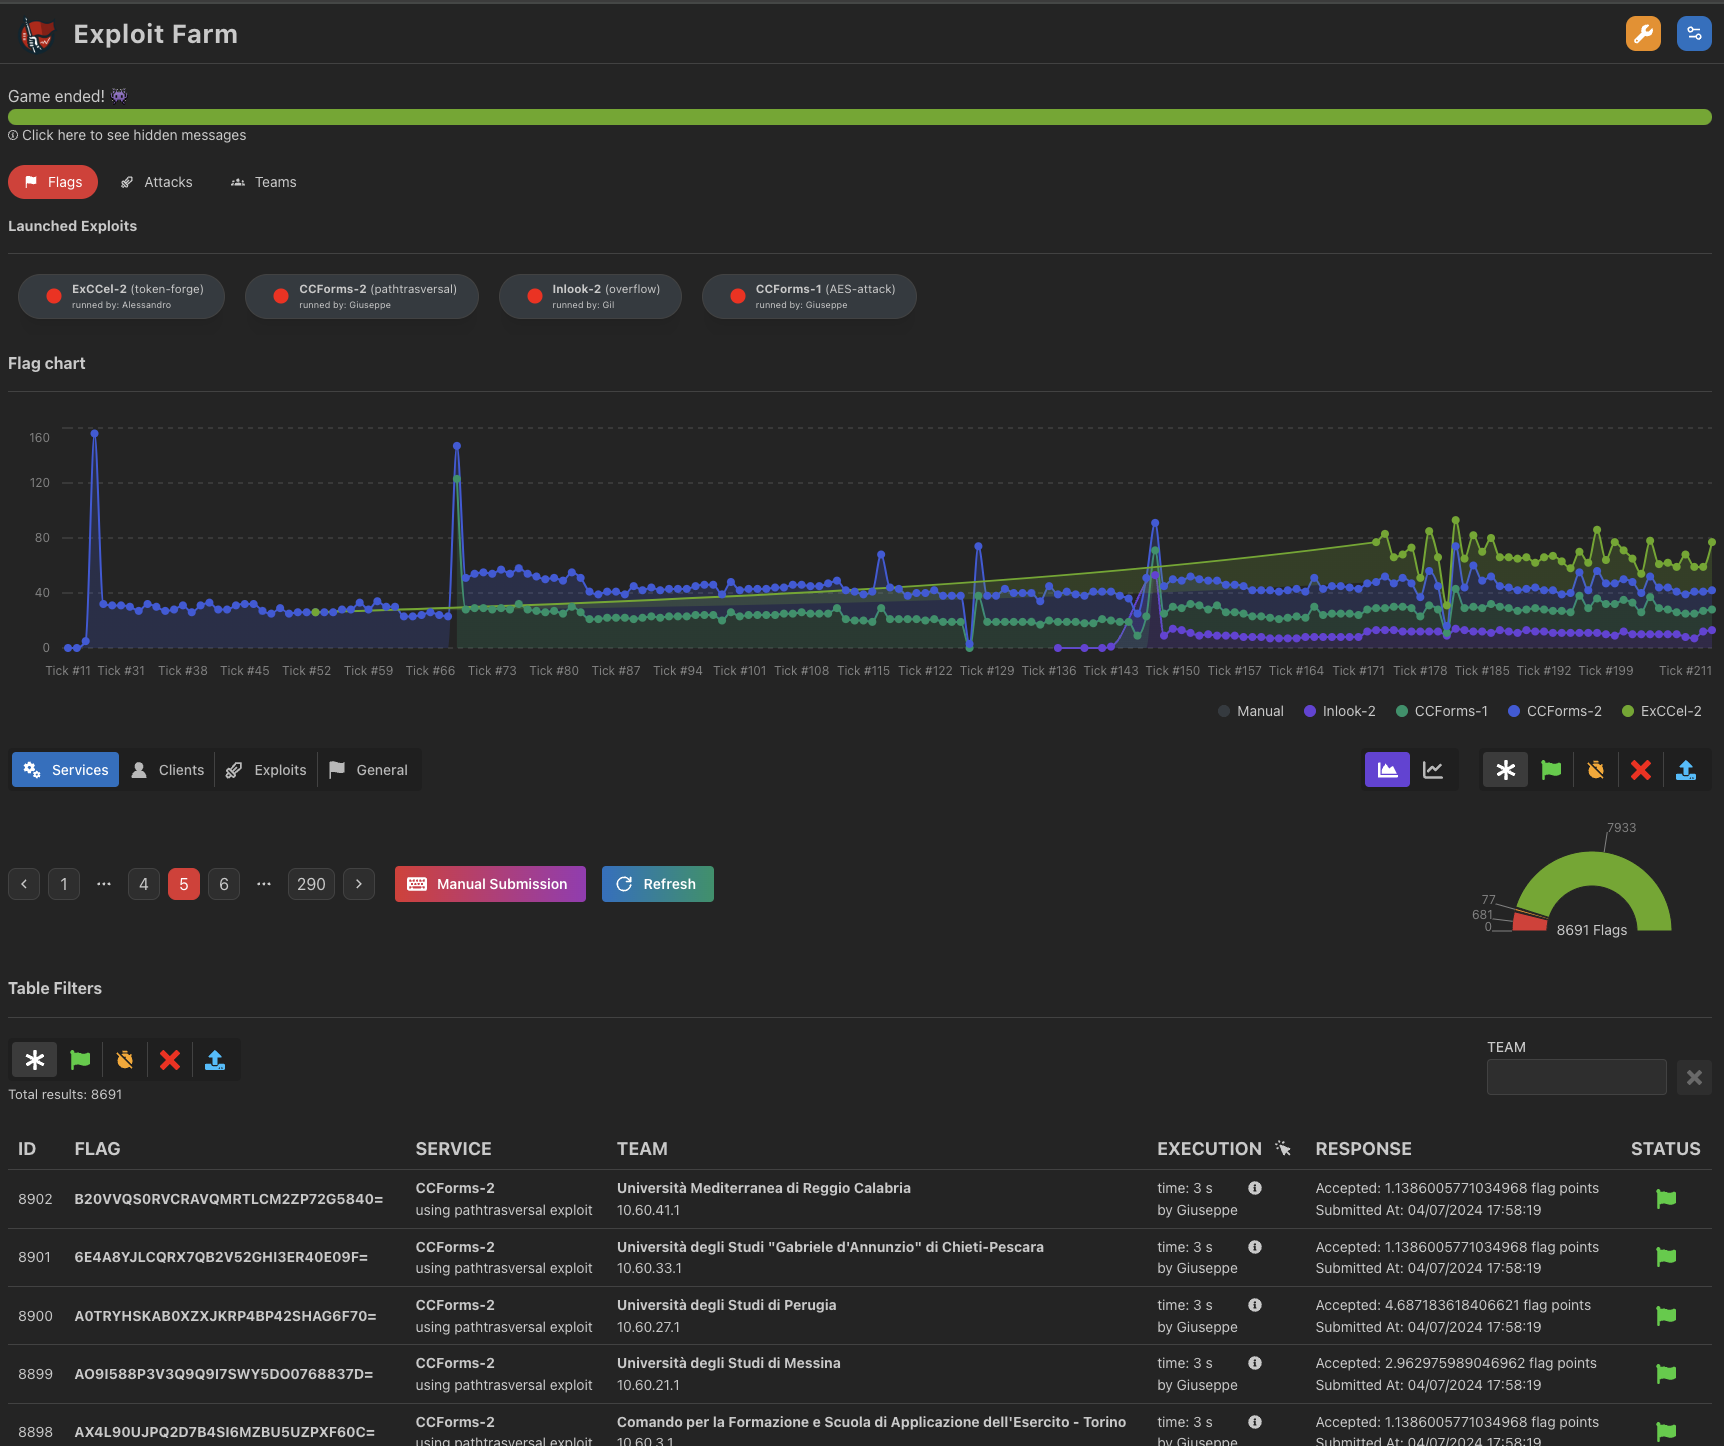
\includegraphics[width=0.8\textwidth]{exploitfarm-web.png}
	\end{figure}
\subsubsection{CLI (xfarm)}
Infine un'ultima parte fondamentale in tutto il progetto è il client che deve essere eseguito preferibilmente su macchine diverse da quella che offre il server, che si occupa dell'esecuzione stessa degli attacchi, della creazione del progetto dell'attacco, del monitoraggio (parziale) dell'attacco stesso. Anche il client stesso dovrà avere un'interfaccia in questo caso TUI intuitiva e veloce da utilizzare che deve rendere immediato e facile l'avvio dell'attacco e l'inserimento dei dati richiesti per l'esecuzione dell'attacco stesso.
    \begin{figure}[H]
    	\centering
    	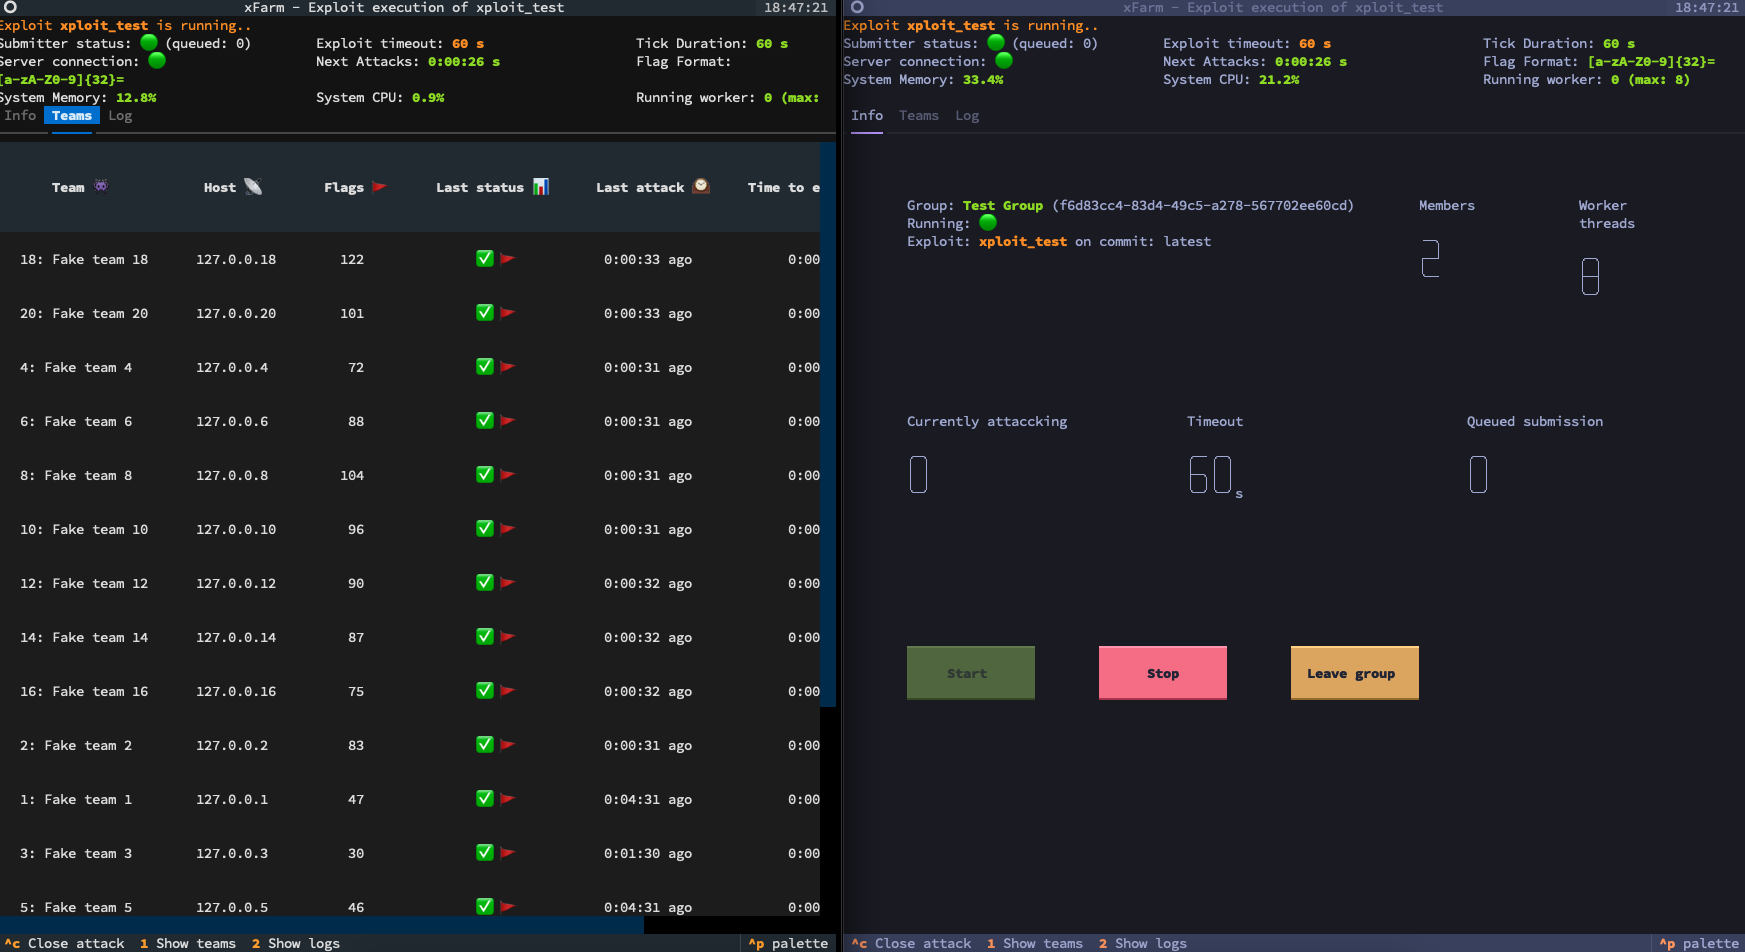
\includegraphics[width=0.6\textwidth]{xfarm-start-cmd.png}
	\end{figure}
\subsection{Specifica dei requisiti}
\subsubsection{Setup}
Il setup di ExploitFarm dalla sua installazione alla conclusione della sua configurazione deve essere di facile ed intuitivo utilizzo e di semplice finalizzazione. Al fine di perseguire questo obiettivo, la tecnologia per l'avvio del progetto è Docker, che ne permette il facile avvio anche del suo database postgres. Inoltre è possibile avviare exploitfarm tramite un one-command, che avvierà il progetto da un repository pubblico con il container buildato. Una volta avviato la configurazione iniziale dovrà essere compilabile sia tramite un'interfaccia web che tramite una automizzazione che è possibile scrivere tramite la libreria python associata al progetto.
\subsubsection{Dinamicità delle configurazioni}
Tutte le configurazioni nella fase di setup devono essere modificabili e automaticamente aggiornate su tutti i client e in tutte le componenti del backend stesso, in modo da evitare interruzioni brusche degli attacchi, permettendo la continuità dell'esecuzione dei client e quindi dispendi di tempo nella riconfigurazione del sistema.
\subsubsection{Gestione Exploit}
I sorgenti degli attacchi devono poter essere facilmente condivisibili e avviabili anche da altri utenti. Inoltre è richiesto anche tenere traccia delle versioni dell'attacco di modo da permetterne la segnalazione di vecchie versioni, aggiornamento di nuove versioni in maniera automatica in caso di attacchi condivisi (definiti in seguito), e analisi post-gara.
\subsubsection{Esecuzione Attacchi}
Gli attacchi devono essere parallelizzati ed eseguiti tenendo conto delle risorse libere nel sistema: in caso il sistema arrivi in trashing o il processore sia saturo, il client deve ribilanciare automaticamente il quantitativo di attacchi eseguiti al fine di non mandare il sistema in blocco.
	\begin{figure}[H]
		\centering
		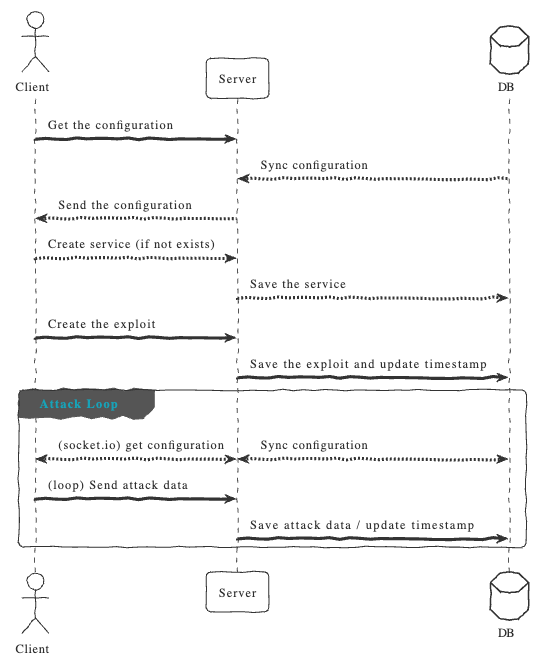
\includegraphics[width=0.45\textwidth]{attack_sequence.png}
	\end{figure}
\subsubsection{Analisi statistiche e visualizzazione}
Il sistema deve disporre di una interfaccia sempre aggiornata e facile da visionare per il monitoraggio delle flag in arrivo, degli attacchi eseguiti, che permetta la visualizzazione degli errori in caso di attacchi crashati o non funzionanti, di selezionare e filtrare i dati in base a dei parametri di ricerca e infine disporre di una serie di grafici che mostrino l'andamento degli attacchi durante la gara, di modo da permetterne una visione immediata.
\subsubsection{Gestione di attacchi distribuiti}
In caso di exploit con un carico computazionale e di memoria non indifferente come nel caso di alcuni attacchi criptografici o di attacchi che necessitano l'elaborazione di media, ExploitFarm deve disporre di un sistema per creare dei gruppi di client che eseguono lo stesso attacco ma i cui team da attaccare siano distribuiti in maniera bilanciata e basata sulla potenza computazionale dei client nel gruppo.
\subsection{Specifiche Tecniche}
\subsubsection{Database}
Il database che gestisce i dati di ExploitFarm, data l'elevata mole di dati aspettata e la velocità di ricerca dei dati richiesta, è postgres e a seguito della stesura dell'analisi dei requisiti è stato progettato seguendo il seguente schema E/R
    \begin{figure}[H]
    	\centering
    	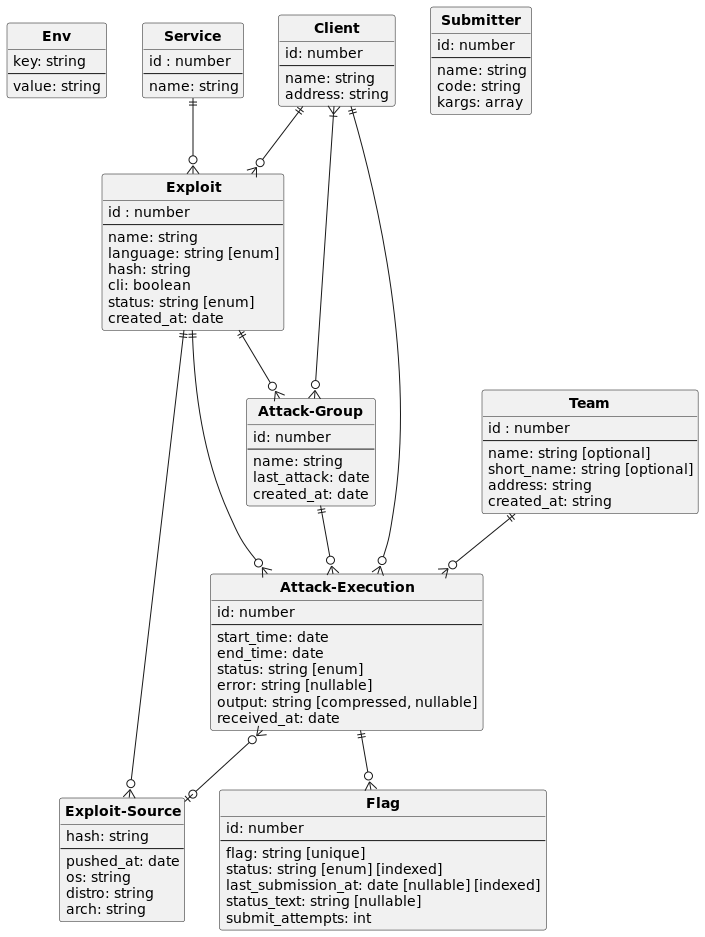
\includegraphics[width=0.6\textwidth]{ExploitFarmDB.png}
	\end{figure}
	Alcune note aggiuntive:
	\begin{itemize}
		\item Env è una tabella che continene alcuni parametri di configurazione di ExploitFarm
		\item è presente una tabella EnvBin nell'implementazione reale ad ora utile solo a scopo di caching e distribuzione della cache delle statistiche
		\item Submitter è una collezione di script python candidati come submitter per il sistema, essendo slegato dalla logica di attacco non ha alcuna relazione con le altre tabelle
	\end{itemize}
\subsubsection{Gestione funzionalità backend}
Il backend di ExploitFarm è composto da 3 parti principali
\begin{itemize}
	\item HTTP API routing and serving
	\item Stats Processor
	\item Submitter Process
\end{itemize}
\paragraph{API HTTP}
L'API HTTP Si occupa di rispondere alle richieste dei client che per la necessità (come da requisito) di mantenere le configurazioni aggiornate, hanno un peso non indifferente sulle richieste fatte, pertanto le API sono parallelizzate per mantenere il sistema reattivo.
\paragraph{Stats processor}
Lo stats processor è nato come necessità dato l'elevato costo computazionale del calcolo dei dati per le statistiche inizialmente affidato alle API HTTP. Lo stats processo in maniera asincrona dal resto del sistema, scarica incrementalmente i dati dal database, e incrementa sempre in maniera scalare un dato strutturato json che contiene i contatori di flag e attacchi sulla base di parametri fortemente eterogenei quali lo stato dell'attacco, lo stato della submission della flag, il team target dell'attacco, il client che ha eseguito l'attacco, il servizio associato e l'exploit associato. La seguente struttura dati ha permesso la generazione dei dati ai fini della creazione dei grafici senza appesantire il sistema ad ogni richiesta dei dati, con la possibilità di eseguire per questo un polling frequente dei dati sia frontend che eventualmente lato client. I dati aggregati con le statistiche vengono compressi e inseriti nel database ad ogni iterazioni, L'API HTTP si limita a scaricare ed esporre i dati. Ci sono particolari casi per modifica di configurazioni per cui lo stats processor ricrea da 0 le statistiche, ma prelevando i dati a blocchi per evitare sovraccarichi, e un ricalcolo stesso incrementale.
\paragraph{Submitter Process}
Il submitter process si occupa della submission delle flag al gameserver dell'infrastruttura di gioco. In particolare rispettando i timeout e le regole configurate nella fase di setup e aggiornando i dati con le ultime modifiche eseguite al submitter anche in fase di esecuzione.
Il submitter inoltre verifica il corretto funzionamento dello script scritto dal team e segnala tempestivamente sia in tutti i client sia nella pagina frontend eventuali errori o warning permettendo al team di verificare e riparare tempestivamente lo script di submission, evitando di perdere punti a causa di errori nella fase di scrittura dello script di submission.
\subsubsection{Funzionalità frontend}
Il frontend deve essere reattivo e dinamico, pertanto utilizza tecnologie come react per la sua realizzazione. Il frontend deve gestire il login alla piattaforma se configurato, eseguire il setup iniziale, offrire un editor per la gestione del submitter, modificare i parametri sulla frequenza di polling dei dati, visualizzazione di grafici, tabella delle ultime flag attenute, visualizzare lo status dei vari exploit, i log dei vari attacchi.
In particolare la schemata principale del frontend deve offrire statistiche tramite grafici su flag, team e attacchi configurabili in base anche a dei filtri nei limiti delle statistiche offerte dal stats processor backend.
\subsubsection{Strutturazione del client (xfarm)}
Il client xfarm è installato nei sistemi tramite la libreria di exploitfarm disponibile sul package manager di python pip, e consiste in una Terminal UI (TUI) che deve permettere la creazione e avvio degli exploit in maniera semplice. In particolare si deve evitare la memorizzazione e l'utilizzo di flag a riga di comando spesso scomodi da utilizzare. xfarm deve richiedere automaticamente la password di autenticazione se richiesta dal backend stesso, chiedere in input e memorizzare in un file di configurazione a livello di utente di sistema, i dati utili alla connessione al backend di ExploitFarm. Queste informazioni devono essere richieste solo una volta, e il client deve automaticamente rilevare il cambio di server exploitfarm tramite un uuid generato dal server per ogni deploy. Inoltre il client deve assicurarsi che la versione del client stesso coincida con quella del server al fine di evitare incongruenze tra client e server. Il client deve anche creare l'ambiente per l'exploit, dove scrivere l'exploit. Il workspace dell'exploit deve essere adatto alla facile pacchettizzazione e auto-avvio dell'attacco anche su altri client. L'exploit deve poter essere scritto per qualsiasi linguaggio, tuttavia ExploiFarm offrirà funzionalità già scritta nella sua libreria per gli script in python dato che rappresenta il linguaggio maggiormente utilizzato per la scrittura di exploit nelle attack defence.
\subsubsection{Autobilanciamento del carico sul client per l'esecuzione degli attacchi}
L'esecuzione degli attacchi agli altri team deve avvenire con un timeout per attacco dinamico e calcolato in base alle risorse della macchina su cui il client è in esecuzione disponibili in realtime, quindi deve adattarsi in base al carico che il sistema ha in quel momento.
\subsubsection{Gestione e versioning degli exploit}
Il client deve permettere l'invio il download e l'update degli exploit caricati sulla piattaforma e di quello presente in locale. Questa funzionalità permette una facile condivisione dei sorgenti degli exploit con gli altri componenti del team ed è fondamentale feature per l'implementazione degli attacchi condivisi.
\subsubsection{Controllo distribuito degli attacchi condivisi}
Il backend tramite anche uno scambio di dati con i client deve bilanciare l'assegnazione dei team ai vari client negli attacchi condivisi senza una configurazione manuale dei pesi sui vari client sulla quantità di team da associare ad ogniuno di questi. Gli attacchi condivisi devono rispettare i cambiamenti di configurazioni e verificare che tutti i client periodicamente, in caso di client non in risposta deve permettere per quanto possibile di portare a termine l'esecuzione di tutti gli attacchi.
\section{Project Managment}
La gestione del progetto è principalmente plan-driven con un approccio però che si avvicina allo "scrum" per progettazione e organizzazione dei task (organizzate in un backlog di user-stories). Il progetto di per se è già in una fase di sviluppo avanzata, pertanto la gestione del progetto riguarderà l'aggiunta della feature per l'avvio di singoli attacchi distribuiti tra più client.
\subsection{Gestione generale}
L'approccio scelto per lo sviluppo delle nuove funzionalità è basato sullo "scrum" con un approccio tendenzialmente plan-driven dati i tempi brevi assegnati per il progetto stesso. Sono assenti le riunioni giornaliere e tutta l'attività si dividerà in soli 2 sprint per l'integrazione di 2 macro-funzionalità.
Sempre a causa di tempi ristretti, i test non sono previsti, ma unicamente micro test durante lo sviluppo stesso per verificarne il funzionamento.
\subsection{Kanban (github)}
Il progetto è interamente condiviso e gestito su github, grazie alla funzionalità dei progetti di cui si sfrutta il backlog che permette di gestire le user-stories con tag, ordini di priorità e direttamente associabili ai branch in cui si esegue l'attività di sviluppo, per questo molto integrato con lo sviluppo stesso.
	\begin{figure}[H]
    	\centering
    	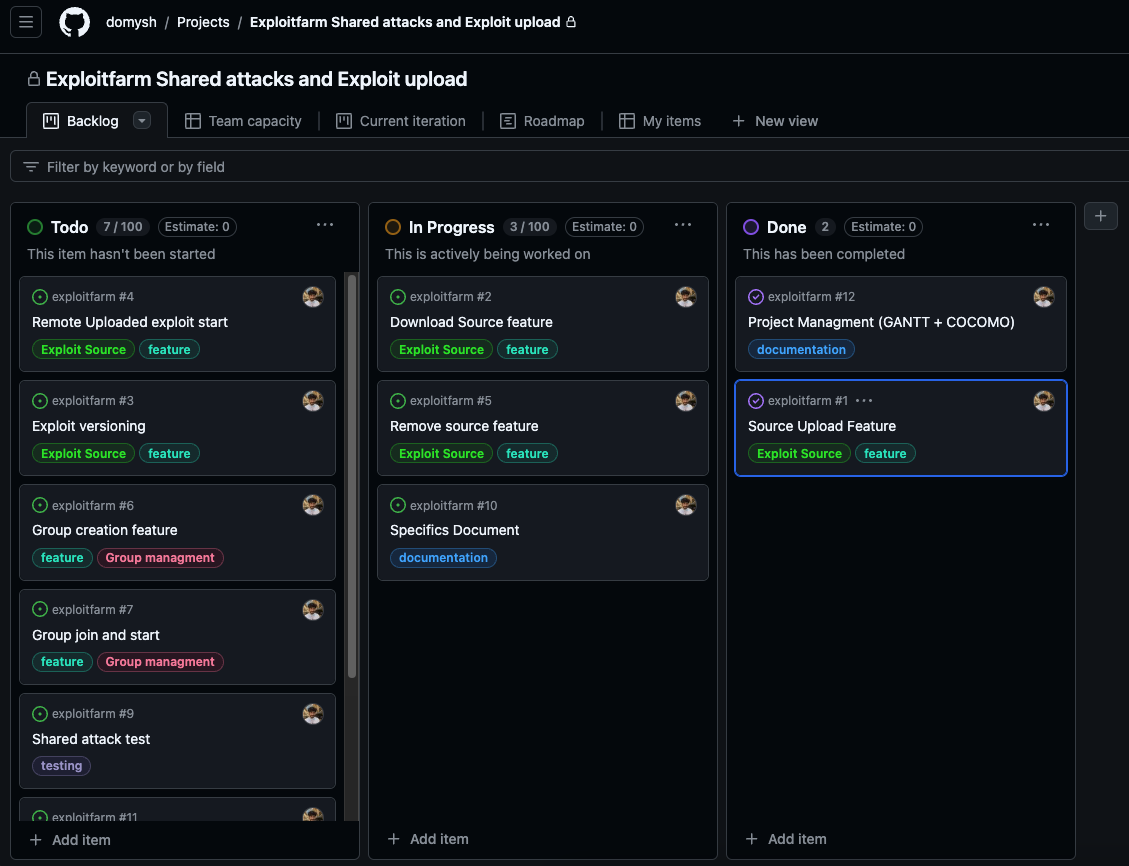
\includegraphics[width=0.6\textwidth]{backlog.png}
	\end{figure}
\subsection{Scheduling}
Sono definite 3 fasi principali nel progetto:
\begin{itemize}
    \item Brainstorming, definizione dei requisiti tecnici e documentazione
    \item 1* Milestone/Sprint: gestione degli exploit
    \item 2* Milestone/Sprint: gestione dei gruppi di client per gli attacchi condivisi
\end{itemize}
Le fasi sono definite proprio per la necessità di progettare lo sviluppo stesso dei nuovi requisiti, e dalla mancanza della feature di gestione degli exploit necessaria allo sviluppo della seconda milestone.
L'inizio del progetto con la prima fase è iniziata il 03-10-2024, la consegna è fissata per il 20-12-2024.
	\begin{figure}[H]
		\centering
    	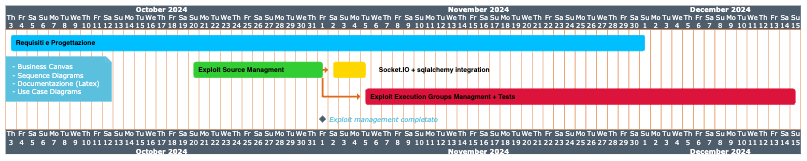
\includegraphics[width=1\textwidth]{scheduling.png}
	\end{figure}
\subsection{COCOMO Analysis}
Il modello COCOMO utilizzato per la stima è quello del Post-architecture model dato che la fase in sviluppo è una fase di implementazione di feature con un progetto di base già pre-ingegnerizzato (Con size stimata di 2k righe di codice).
   \[ E = A \times Size^B \times \prod_{i=1}^{n} EM_i \]
   Con:
   \[ B = 0.91 + 0.01 \times \sum Scale Factors \]
   \begin{itemize}
   		\item A = 2.94 (tipico per Post-Architecture COCOMO)
		\item $Size \simeq 2k$ righe di codice
   \end{itemize}
\subsubsection{Effort Multipliers}
Si utilizzerà un subset dei 17 moltiplicatori previsti per COCOMO post-architecture.
\begin{itemize}
	\item RELY = 1.26 (Very High)
	\item DATA = 1.00 (Nominal)
	\item CPLX = 1.17 (High)
	\item RUSE = 0.95 (Low)
	\item DOCU = 1.00 (Nominal)
	\item TIME = 1.29 (Very High)
	\item PVOL = 1.00 (Nominal)
	\item PCAP = 0.88 (High)
	\item TOOL = 0.90 (High)
	\item SITE = 1.00 (Nominal)
	\item SCED = 1.00 (Nominal)
\end{itemize}
	\[
		\prod_{i=1}^{n} EM_i = 1.431
	\]
\subsubsection{Scale Factors}
\begin{itemize}
	\item PREC = 1.24 (Very High)
	\item FLEX = 1.01 (Very High)
	\item RESL = 4.24 (Nominal)
	\item TEAM = 1.0 (No team, not used)
	\item PMAT = 1.56 (Very High)
\end{itemize}
   \[ B = 0.91 + 0.01 \times \sum Scale Factors = 0.99 \]
\subsubsection{Risultato Finale}
   \[ E = A \times Size^B \times \prod_{i=1}^{n} EM_i = 8.36 \]
\subsubsection{Duration}
   \[ C = 3.67 \]
   \[ D = 0.28 + 0.2 \times (B - 0.91) = 0.296 \]
   \[ T = C \times E^D = 6.8 (mesi) \]
   Tuttavia assumendo gli obiettivi del progetto, è intuitivo comprendere come la stima eseguita è eccessiva rispetto al reale tempo necessario al raggiungimento dell'obiettivo.
\subsection{Risk Managment and Analysis}
\subsubsection{Stima dell'Effort e requisiti}
Durante lo sviluppo c'è la possibilità nascano nuove esigenze date da limitazioni tecniche attualmente presenti nel progetto: per attutire i danni possibili generati dalla nascita di nuovi requisiti o anche alla sottostima del tempo necessario, è necessario iniziare al più presto dalla data schedulata l'effettiva data di inizio dello sviluppo di modo da permettere l'allocazione di più slot temporali ad una determinata user-story nello sviluppo prima che possa terminare la deadline di consegna, punto critico nel progetto. Il livello di rischio associato è "Moderato".
\subsubsection{Rilascio di versioni non totalmente funzionanti}
C'è la possibilità che a causa di modifiche a diverse parti del progetto, si possano presentare bug in parti non direttamente inerenti ma collegate alla parte di software modificata. Per ovviare a questo problema è utile eseguire in maniera atomizzata prima della pubblicazione della release dei test automatici che verificano il funzionamento corretto della piattaforma. Nonostante il rischio si classificato come Medio, date le scadenze strette non è prevista attualmente la scrittura di test automatizzati.
\subsubsection{Rischio di rendere la piattaforma complessa gestire}
Il progetto ha grandi requisiti e grandi ambizioni a livello di funzionalità che tuttavia dopo essere sviluppate possono risultare complesse nel loro utilizzo anche per gli utenti target che sono classicamente utenti esperti. Andando in questa direzione potremmo perdere uno degli obiettivi del progetto, cioè quello di facile utilizzo, autorizzazione e setup. Il rischio è medio elevato e potrebbe comportare lo sviluppo di parti della piattaforma che necessitano un completo refactoring o riscrittura in seguito. Per evitare questo rischio è necessario un confronto esterno con altri giocatori CTF per avere opinioni esterne, quindi opinioni esenti del bias dello sviluppatore del progetto, che sviluppandone le funzionalità non si rende conto di eventuali funzionalità complesse da utilizzare. Questo permetterebbe una rivisitazione e progettazione migliore del progetto.
\subsection{Release Managment}
Le release di ExploitFarm avvengono tramite github con una catena di building automatica del container di exploitfarm che contiene frontend compilato e backend, automaticamente rilasciato e pubblicato su gihtub packages che ne rilascia il download pubblico.
Inoltre per l'esecuzione di exploitfarm è disponibile uno script che genera dinamicamente un docker compose e lo avvia utilizzando i container pullati dai repository online, e inoltre si assicura che la versione avviata di exploitfarm sia l'ultima disponibile.
\subsection{Modello di Business}
Il progetto di per se nasce come progetto totalmente opensource, quindi non a scopo di lucro. Tuttavia un possibile approccio di Business adottabile liberamente ispirato a quello di un'altra importante piattaforma opensource per le competizioni CTF Jeopardy (\href{https://github.com/CTFd/CTFd}{CTFd}) è quello di continuare ad offrire una piattaforma completamente opensource e gratuita ma di offrire a pagamento un deploy di ExploitFarm con eventuali client attaccanti hostati (con dimensioni del server adattabili e scalati anche in base al costo e al peso dell'exploit) di modo da rendere immediato l'accesso all'attacker, anche con eventuali supporti rapidi alla connessione a VPN della gara, o al bridging da uno dei PC del team della rete di gara se non sono presenti connessioni VPN.
\section{Analisi SWOT}
\subsection{S: Punti di forza}
\begin{itemize}
	\item Unicità sulle funzionalità
	\item Interfaccia innovativa
	\item Setup Semplice
	\item TUI
	\item Statistiche
\end{itemize}
\subsection{W: Punti di debolezza}
\begin{itemize}
	\item Elevata complessità
	\item Centralizzato (SPOF)
\end{itemize}
\subsection{O: Opportunità}
\begin{itemize}
	\item Pubblicizzazione
	\item Aggiunta di test automatici
\end{itemize}
\subsection{T: Minaccie}
\begin{itemize}
	\item Impossibilità di mantenere il progetto a fronte di una grande complessità da gestire
\end{itemize}
\section{Sviluppi Futuri}
\begin{itemize}
	\item eliminare come single point of failure il server e permettere l'esecuzione di backend multipli e decentralizzati così da evitare in caso di problemi con uno dei server. La gestione di backend decentralizzati è di una complessità altissima e non strettamente necessario per gli obiettivi del progetto pertanto si lascia come sviluppo futuro.
\end{itemize}
\end{document}
